\section{Test/Resultater}

I dette afsnit beskrives der nogle af de tests, vi lavede for både at debugge, men også for at indsamle data, der skulle bruges for at komme videre med programmeringen.

\subsection{Bremse-test}

For at teste effekten af bremsen, opstillede vi en lang lige bane, for at afprøve bilens bremselængde. Bremselængde skulle gerne variere alt efter, hvor lang tid motoren var kortsluttet. Vi satte bilen igang med samme hastighed, og varierede kortslutningsperioderne i intervallerne 0, 50, 100, 200, 300, 400 og 500 millisekunder. Når bilen krydsede målstregen, slukkedes motoren, og bremsen blev tilsluttet. Så lod vi bilen køre indtil den stoppede, og målte afstanden til målstregen. Hver periode blev kørt fem gange, og så beregnede vi gennemsnittet. Testen blev lavet for tre forskellige værdier i OCR2 - 255, 180 og 120 svarende til duty cycles på henholdsvis 100 \%, 70,6 \% og 47 \% (se figur \ref{fig:Bremselir}). 

\begin{figure}[h]

	\centering
		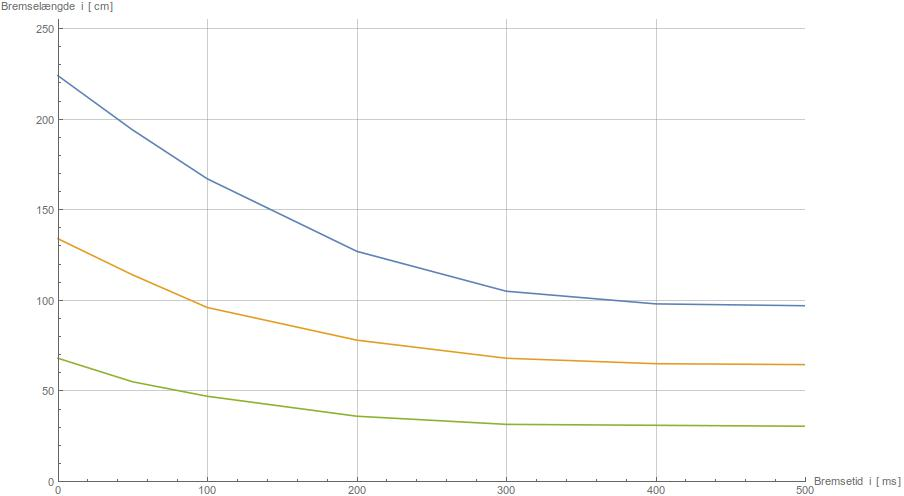
\includegraphics[scale=0.4]{Billeder/Bremse.jpeg}
	\caption{Her ses bremselængden i forhold til bremsetiden, med bremselængden i cm op ad y-aksen, og bremsetiden i ms ud ad x-aksen}
	\label{fig:Bremselir}
	
\end{figure}

Ud fra testen kan vi konkludere, at bremsen har størst effekt ved korte bremsetider under 300 ms.

\pagebreak

\subsection{Databehandling vha. bluetooth}

Vi lavede også en række tests, hvor vi brugte bluetooth modulet til at sende data til et terminalprogram, så vi kunne plotte eksempelvis gyrodata i en graf (se figur \ref{fig:Gyro}). Ud fra en graf var det nemmere at afgøre helt præcist, hvordan dataen skulle behandles i programmet. Vi lavede også tests, hvor vi plottede OCR2 sammen med den målte "hastighed", for at evaluere hastighedskontrollen tidligt i udviklingen.

\begin{figure}[h]

	\centering
		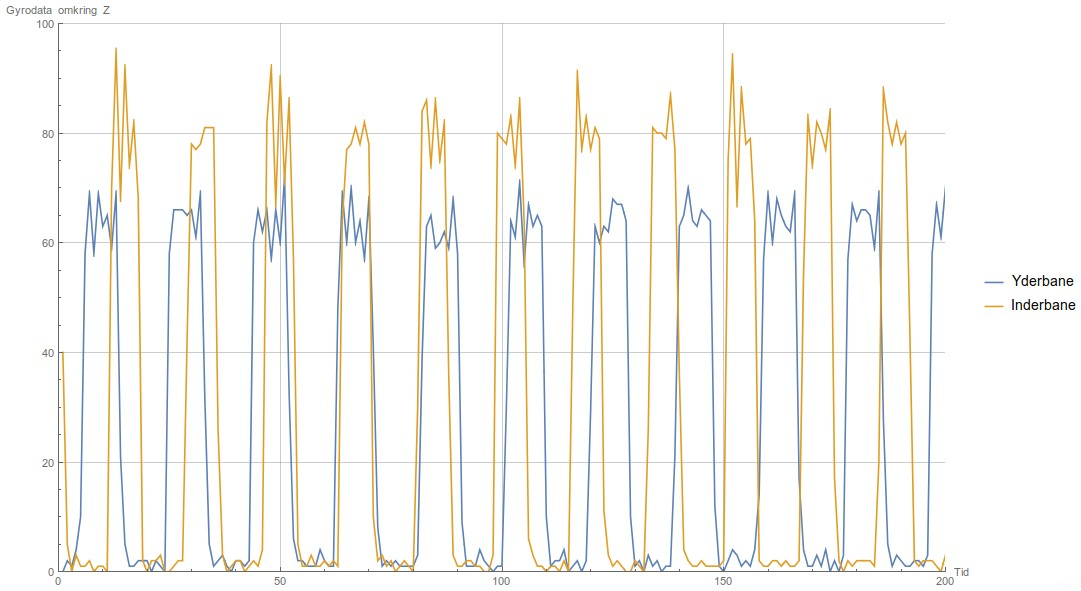
\includegraphics[scale=0.4]{Billeder/Gyro.jpg}
	\caption{Her ses forskellen mellem vinkelaccellerationen på yder- og inderbanesving ved nogenlunde konstant hastighed}
	\label{fig:Gyro}
	
\end{figure}

\subsection{Mapping-test}
\begin{wrapfigure}{l}{6cm}
	\begin{minipage}{.3\textwidth}
	\centering
		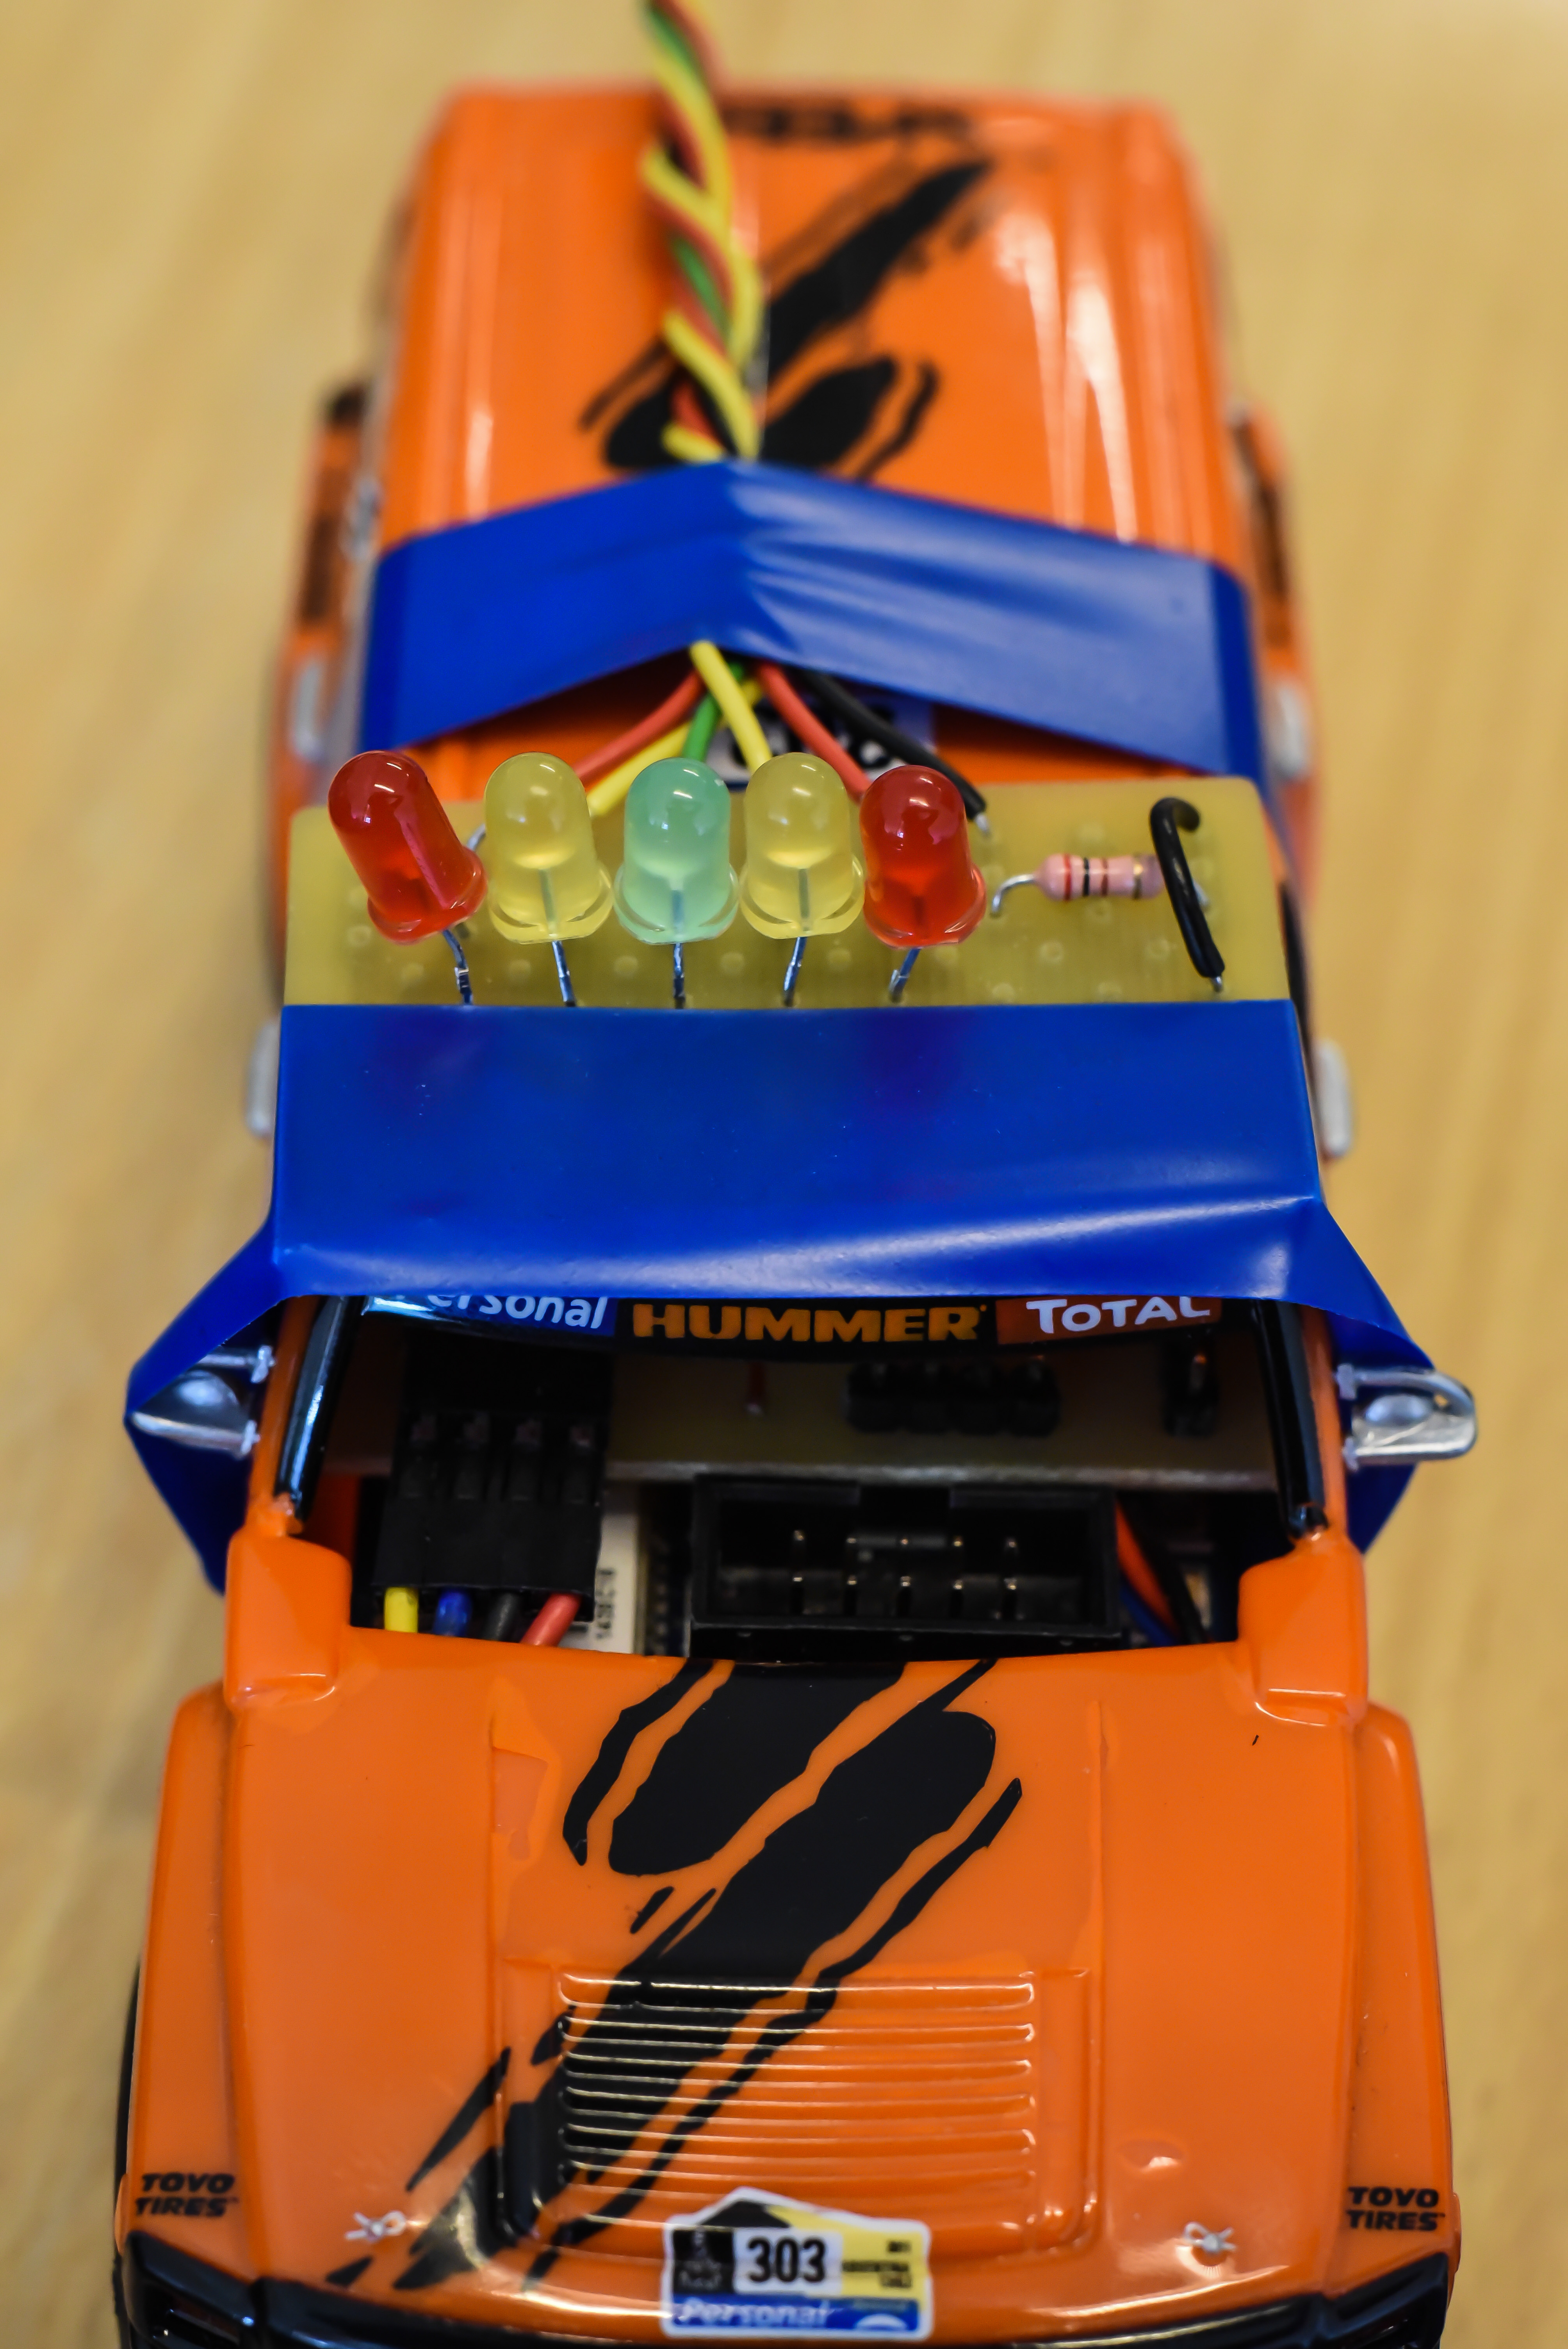
\includegraphics[scale=0.02]{Billeder/Debug-lys.JPG}
	\caption{Her ses vores debugging-LED'er monteret på bilen.}
	\label{fig:Udrykning}
	\end{minipage}
\end{wrapfigure}
Til at fintune gyro-værdierne for sving og afprøve om baneelementerne blev mappet korrekt, fastmonterede vi fem LED'er, vi kunne tænde individuelt så, det var muligt at se direkte, om microcontrolleren reagerede, som vi ville have den til (se figur \ref{fig:Udrykning}).

Hver LED fik sit eget IO-ben, og så \\ blev de tændt alt efter hvilken værdi, gyroen sendte tilbage, således at de røde LED'er repræsenterede yderbanesving, de gule: inderbanesving og den grønne: ligeud. På den måde kunne man nemt se, hvordan bilen tolkede banen under mappingrunden, og om værdierne blev gemt rigtigt i SRAM-hukommelsen.	Eksempelvis havde vi et problem, hvor microcontrolleren gemte det sidste baneelement på den forkerte RAM-addresse - det var nemt at se fordi, den lige i det tilfælde, konsekvent troede at der var et lige baneelement et sted på banen, hvor der var et sving. Derudover kunne LED'erne bruges til at teste andre funktionaliteter, som for eksempel hvornår bremserne blev slået til, hvornår der blev givet fuld gas osv.